\documentclass[onecolumn]{article}

%Titling
    \usepackage[compact]{titlesec}
    \titlespacing{\section}{0pt}{3ex}{2ex}
    \titlespacing{\subsection}{0pt}{2ex}{1ex}
    \titlespacing{\subsubsection}{0pt}{1ex}{0.5ex}
\titleformat*{\section}{\Large\scshape}
\titleformat*{\subsection}{\Large}
\titleformat{\subsubsection}[runin]
  {\normalfont\bfseries}{\thesubsection}{1em}{}
  
%Page size
	\addtolength{\oddsidemargin}{-.875in}
	\addtolength{\evensidemargin}{-.875in}
	\addtolength{\textwidth}{1.75in}

	\addtolength{\topmargin}{-.875in}
	\addtolength{\textheight}{1.75in}
	
	\parskip=.1cm
	
%Indented paragraph
\setlength{\parindent}{0pt}
\newenvironment{indentpar}[1]
  {\begin{list}{}
          {\setlength{\rightmargin}{#1}}
          \item[]
  }
  {\end{list}}

\usepackage{graphicx}
\graphicspath{ {figures/} }
\usepackage[T1]{fontenc}
\usepackage{lmodern}
\usepackage{float}
\usepackage[table]{xcolor}
\usepackage{multirow}
\usepackage{tabularx} 
\usepackage[table]{xcolor}
\usepackage[font=small,labelfont=bf]{caption}
\usepackage{textcomp}
\usepackage{gensymb}
\usepackage{lineno}
\usepackage{amsmath}
\usepackage{blindtext}
\usepackage{texshade}
\usepackage{bigdelim}
\usepackage{textgreek}
\usepackage{multicol}

% tikz setup
\usepackage{tikz}
\usetikzlibrary{shapes,arrows}
\newcommand*{\h}{\hspace{5pt}}% for indentation
\newcommand*{\hh}{\h\h}% double indentation


%Citations
\usepackage[authoryear]{natbib}
\setcitestyle{authoryear,open={(},close={)}}
\renewcommand{\bibname}{References}

\usepackage[allbordercolors = white, linkcolor = blue, citecolor = blue, colorlinks = true]{hyperref}
\usepackage[nameinlink]{cleveref}

%titling
\title{Models of readmission to intensive care units perform poorly in external validation}
\author{Ben Cooper$^1$, Simon Howell$^{1,2}$, Alwyn Kotzé$^{1,2}$, Tom Lawton$^3$, Peter Tennant$^1$, David Wong$^4$}
%1 University of Leeds, 2 Leeds Teaching Hospitals NHS Trust, 3 Bradford Teaching Hospitals NHS Trust, 4 University of Manchester

\date{%
    $^1$University of Leeds, $^2$Leeds Teaching Hospitals NHS Trust, $^3$Bradford Teaching Hospitals NHS Trust, $^4$University of Manchester\\[2ex]%
    \today
}



\begin{document}
\maketitle

\section{Introduction}

% Brief background on ICU risk stuff
Unplanned readmission to an intensive care unit (ICU) during the same hospital admission is a relatively common event, affecting between 1.3\% and 13.7\% of all ICU patients \citep{Elliott2014}. Not only do readmissions to ICU represent a substantial strain on hospital resources, but also readmitted patients tend to have worse prognoses, increased length of ICU stay, and greater risks of morbidity and mortality \citep{MarkaziMoghaddam2020}. Despite this, the precise factors contributing to ICU readmission risk remain unclear. Several models for risk prediction have been developed which tend to use very different variable sets, and no model has been widely externally validated. In this study, we aimed to use two independent datasets to externally validate several major readmission risk models and make recommendations for future work in this field.

\section{Methods}

\subsection{Data Sources}

This study used two independent data sets: The open-access MIMIC-III critical care database \citep{Johnson2016}, and a dataset of ICU patients  from Leeds Teaching Hospitals NHS Trust, UK (LTH. MIMIC-III  comprises ICU stay information for 61,532 adult patients at the Beth Israel Deaconess Medical Centre between June 2001 and October 2012. The MIMIC dataset includes information such as demographics, vital sign measurements made at the bedside ($\sim$1 data point per hour), laboratory test results, procedures, medications, caregiver notes, imaging reports, and mortality (both in and out of hospital). The LTH dataset contains the variables proscribed by the UK Intensive Care National Audit and Research Centre (ICNARC) which cover medical history, demographics, ICU stay descriptors and the worst values of a range of physiological variables during the patient's first 24 h in ICU.

\subsection{Inclusion criteria and outcome measure}

% Workflow in extract_patients & preprocess_data
An overview of inclusion and exclusion criteria is shown in \Cref{FlowchartMIMIC} and \Cref{FlowchartICNARC}. For the MIMIC dataset, we selected all patients admitted under a surgical service who underwent an elective surgical procedure, followed by an ICU stay. Patients with missing data for variables required by risk estimation models, or patients who died in ICU were excluded. A similar process was followed for the LTH ICNARC data, where we included all patients who underwent a planned, elective surgical procedure, followed by an ICU stay. Final sample sizes used for model validation were n = 2,152 for the MIMIC dataset and n = 1,828 for the ICNARC dataset.

The `readmission' outcome measure for both datasets was defined as patients readmitted to the ICU within 30 days of discharge from ICU. This covers both patients fully discharged from hospital then readmitted to ICU, and patients discharged to lower wards then readmitted to ICU without leaving hospital. This resulted in a readmission rate of 8.7\% (n = 187 patients) in the MIMIC dataset and 3.8\% (n = 70 patients) in the ICNARC dataset.

% Flowchart------------
\begin{figure}[t]
\centering
	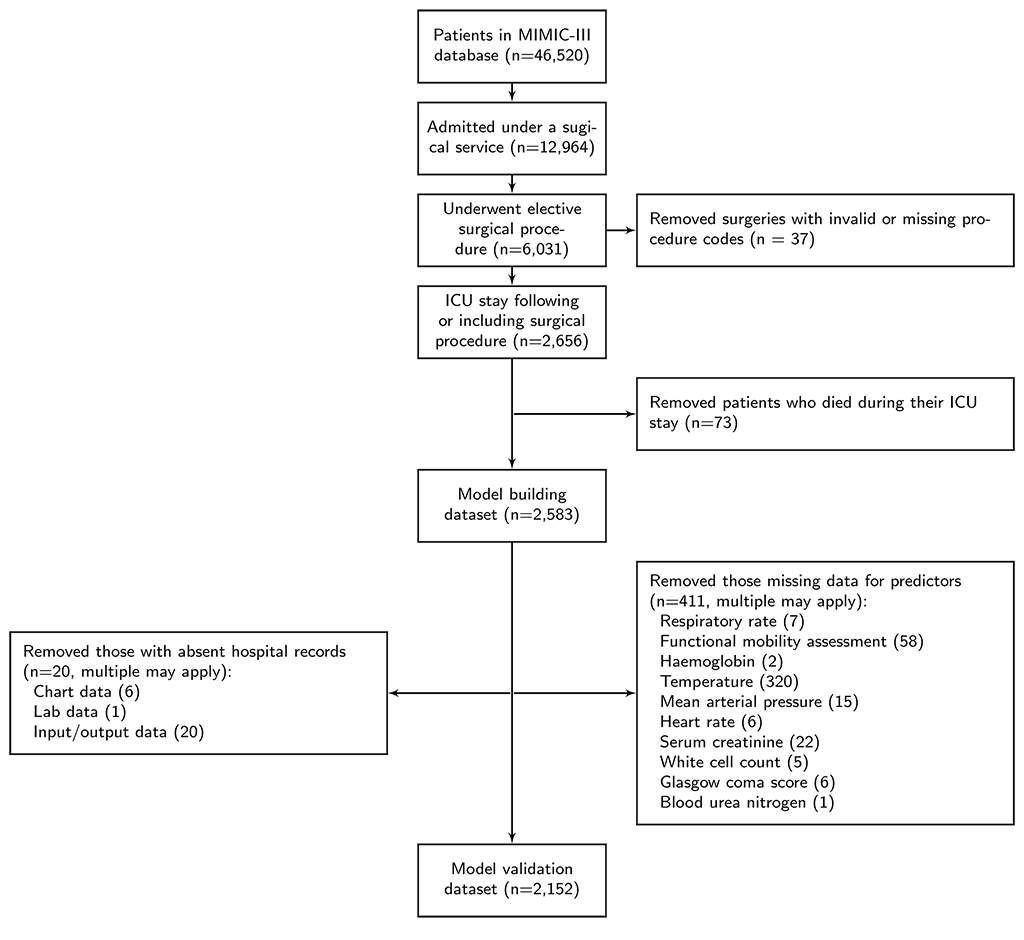
\includegraphics[width=\textwidth]{flowchart_mimic.png}
  \caption{Flowchart of inclusion and exclusion criteria for patients in the MIMIC-III dataset, alongside sample sizes at each step.}
  \label{FlowchartMIMIC}
\end{figure}


\subsection{Candidate models}

Here, we give an brief overview of each model, as well as the model performance metrics given in the paper deriving each model. In general, the performance of binary prediction models can be measured in two separate but related metrics using an unseen validation dataset. Discrimination is usually measured as the area under the Receiver Operating Characteristic curve (called AUROC or AUC). It measures the model's ability, when presented with two patients, one of whom was readmitted and one of whom was not, to assign a greater probability of readmission to the patient who was ultimately readmitted. Its values range from 0.5, indicating a model no better than guessing, to 1, indicating perfect discrimination. Crudely, discrimination can be classified as poor (0.5--0.6), moderate (0.6--0.7), good (0.7--0.8), very good (0.8--0.9) and excellent (>0.9).

Calibration measures the agreement between a model's predicted readmission, and observed readmission. This is usually performed by splitting patients into deciles based on assigned readmission probability, then comparing observed to expected readmission rates within each decile. This goodness-of-fit can then be formally assessed using a Hosmer-Lemeshow Chi-squared ($ \chi^{2} $) test, with a well-calibrated model showing no significant differences between observed and expected readmission. \Cref{Table1} cross-tabulation of each model's predictors with readmission status from the MIMIC and ICNARC datasets, to demonstrate the expected relationship between each predictor and readmission.

% Flowchart------------
\begin{figure}[h]
\centering
	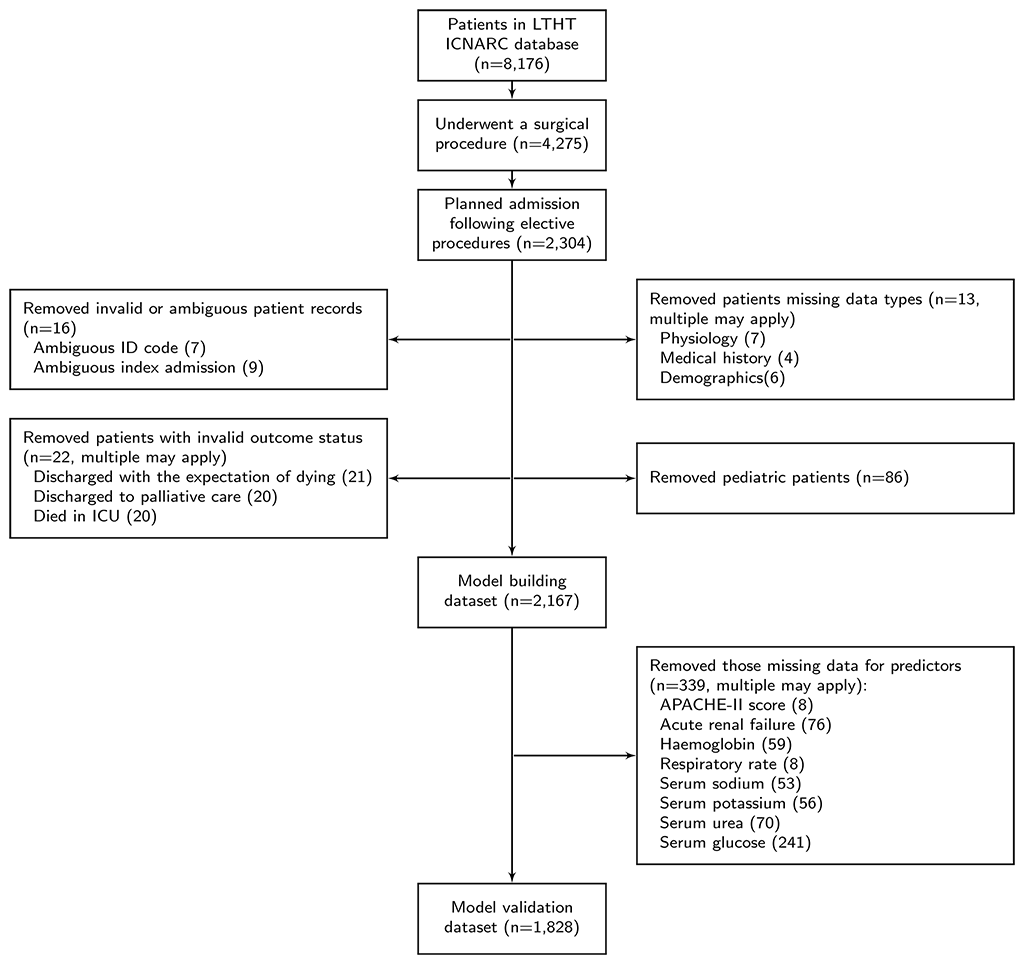
\includegraphics[width=\textwidth]{flowchart_icnarc.png}
  \caption{Flowchart of inclusion and exclusion criteria for patients in the LTH ICNARC dataset, alongside sample sizes at each step.}
  \label{FlowchartICNARC}
\end{figure}

\begin{table*}
\centering
	\renewcommand{\arraystretch}{1.4}
		\caption{Cross-tabulation of variables in each ICU readmission risk prediction model with ICU readmission status in the MIMIC-III and LTH ICNARC datasets. Continuous variables are presented as means $\pm$ standard deviation. Fluid balance information was unavailable in the LTH dataset.}
	\begin{tabular}{lp{2.5cm}p{3cm}p{2.5cm}p{3cm}}
		\hline
		& MIMIC-III & & ICNARC &\\
		& No Readmission & Readmitted to ICU & No Readmission & Readmitted to ICU\\
		\hline
		N & 1965 (91.3\%)  &    187 (8.7\%) & 1758 (96.2\%) & 70 (3.8\%)\\
		\cite{Frost2010} &&&&\\
		Age & 63.4 $\pm$ 13.6 & 66.7 $\pm$ 12.7 & 62.6 $\pm$ 14.5 &  63.2 $\pm$ 14.9 \\
		Sex &&\\
		\quad Male & 1212 (61.7\%)   &    126 (67.4\%) & 1042 (59.3\%) & 40 (57.1\%)\\
		\quad Female & 753 (38.3\%)  &     61 (32.6\%) & 716 (40.7\%) & 30 (42.9\%)\\
		Admission source &&\\
		\quad Operating theatre & 1957 (99.6\%)  &   185 (98.9\%) & 1757 (99.9\%) & 70 (100\%)\\
		\quad Other hospital & 6 (0.3\%)    &    2 (1.1\%) & 0 (0\%) & 0 (0\%)\\
		\quad Ward & 2 (0.1\%)   &     0 (0\%) & 1 (0.1\%) & 0 (0\%)\\
		APACHE-II score & 21.5 $\pm$ 8.26 & 22.5 $\pm$ 7.72 & 10.6 $\pm$ 3.80 & 12.0 $\pm$ 3.68 \\
		ICU stay >7 days & 151 (7.7\%)   &     22 (11.8\%) & 45 (2.6\%) & 5 (7.1\%)\\
		Discharged after hours & 1025 (52.2\%)    &   105 (56.1\%) & 665 (37.8\%) & 31 (44.3\%)\\
		Acute renal failure & 130 (6.6\%)   &    38 (20.3\%) & 249 (14.2\%) & 10 (14.3\%)\\
		\cite{Martin2018} &&&&\\%%%%%%%%%%%%
		Respiratory rate & 17.8 $ \pm $ 3.55 & 18.5 $ \pm $ 3.73 & 22.4 $\pm$ 4.10 & 21.9 $\pm$ 3.76 \\
		Blood urea nitrogen (mg/dl) & 18.2 $ \pm $ 10.3 & 19.6 $ \pm $ 10.8& 17.8 $\pm$ 8.48 & 18.1 $\pm$ 7.62 \\
		Serum glucose (mg/dl) & 158.3 $ \pm $ 40.6 & 158.4 $ \pm $ 42.2& 179.8 $\pm$ 48.1 & 186.1 $\pm$ 47.4 \\
		Serum chloride (mmol/L) & 108.6 $ \pm $ 4.54 & 107.9 $\pm$ 5.05 & 101.2 $\pm$ 3.53 & 100.3 $\pm$ 3.35 \\
		History of atrial fibrillation& 584 (29.7\%) &  78 (41.7\%) & 36 (2\%) & 2 (2.9\%) \\
		History of renal insufficiency &61 (3.1\%) & 3 (1.6\%) & 38 (2.2\%) & 2 (2.9\%) \\
		\cite{Hammer2020}&&&&\\%%%%%%%%%%%%%%%%
		General surgery & 306 (15.6\%) & 40 (21.1\%) & 29 (1.6\%) & 1 (1.4\%) \\
		Cardiac surgery & 1038 (52.8\%) & 81 (43.3\%) & 325 (18.5\%) & 14 (20\%) \\
		Hyperglycaemia (>180 mg/dl) & 425 (21.6\%) & 47 (25.1\%) & 715 (40.7\%) & 30 (42.9\%) \\
		Severe anaemia (<7 g/dl) & 602 (30.6\%) & 57 (30.5\%) & 248 (14.1\%) & 16 (22.9\%) \\
		APACHE-II > 20 &  1190 (60.6\%) &  110 (58.8\%) & 33 (1.9\%) & 2 (2.9\%) \\
		Positive fluid balance >5L & 176 (9\%)  & 36 (19.3\%) & \textit{N/A} & \textit{N/A} \\
		No ambulation & 1486 (75.6\%) & 149 (79.7\%) & 849 (48.3\%) & 41 (58.6\%) \\
		ICU stay >5 days & 245 (12.5\%) &  34 (18.2\%) & 135 (7.7\%) & 16 (22.9\%) \\
		\hline
	\end{tabular}
	\label{Table1}
\end{table*}


\subsubsection*{Frost.}

\cite{Frost2010} used a logistic regression model to develop a nomogram for predicting ICU readmission risk based on 14,952 patients in a single hospital in Australia. As they do not present the coefficients from their model directly, only in the form of the nomogram, several of these coefficients can only be approximated, which may hinder external validation of the model.

The Frost model includes the following variables: Age, sex, elective admission (yes/no), admission source (Operating theatre/recovery ward, emergency department, other hospital or general ward), APACHE-II score at discharge, ICU stay duration > 7 days (yes/no), discharge outside the hours of 08:00--16:00, and acute renal failure during ICU stay (yes/no). Each variable carries a number of points, the sum of which is used to determine readmission risk. For validation, we did not use the "elective admission" variable, as all admissions in our datasets were elective. For similar reasons, almost all admissions were from the operating theatre.  The binary `acute renal failure' flag was not available in the ICNARC dataset. Thus, we used the MIMIC dataset to build a model predicting acute renal failure from serum creatinine concentration and urine output, and used this model to estimate acute renal failure for each patient in the ICNARC dataset.

Unfortunately, the coefficients linking variables to score, and total score to readmission risk are not presented, and must be inferred from the nomogram. In most cases, variables map clearly onto discrete score values. However, the mapping between total score and readmission is neither linear nor exponential. Here, we approximate the mapping from the points scale to predicted readmission using a logarithmic relationship. This approximation may result in poor calibration of the Frost model. The authors report moderate discrimination (AUC = 0.66), and do not quantitatively report calibration, only describing it as `good'.




\subsubsection*{Martin.}

\cite{Martin2018} also developed their model into a nomogram, but unlike Frost, also provided coefficients and a precise formula to generate risk estimates. Their model used 3,109 patients in a single academic centre, and narrowed an initial 179 candidate variables down to 7 variables: Age, respiratory rate, blood urea nitrogen concentration, serum glucose, serum chloride, history of atrial fibrillation (yes/no) and history of renal insufficiency (yes/no). Serum chloride concentration was not available in the ICNARC dataset, and so was estimated from serum sodium and serum potassium concentrations with a model developed using the MIMIC dataset.

The Martin model was built with any readmission to ICU within 72 h of discharge as the outcome measure. It used the least absolute shrinkage and selection operator (lasso) approach to regression, which aims to reduce very small coefficents to zero, thus performing automated feature selection. The authors report good discrimination (AUC = 0.71), and whilst they claim in the methods that `...the model's goodness of fit of was assessed using the Hosmer-Lemeshow test', no calibration results are reported statistically or visually.

\subsubsection*{Hammer.}

Finally, \cite{Hammer2020} developed the `RISC' score (Readmission to the Intensive care unit in Surgical Critical care patients, henceforth simply called `Hammer' for consistency with other models) using logistic regression. Their model aimed to include a number of binary, modifiable variables to aid its use as a clinical tool.

The Hammer model is a logistic regression model with the specific goal of including modifiable predictors, to increase the model's usability as a clinical tool. It was built using 7,126 patients from the same medical centre that the MIMIC-III database comes from, though the data collection dates do not overlap. To further aid clinical usage, the model contains only binary yes/no variables: Sex, general surgical procedure, cardiac surgical procedure, APACHE-II score of >20 on admission, ICU stay of >5 days, positive fluid balance >5L throughout ICU stay and, within the last 24 h, hyperglycaemia, severe anaemia and no ambulation. Ambulation status was approximated in the ICNARC dataset by whether the patient was expected to have any dependency post-discharge. No suitable proxy for fluid balance existed in the ICNARC dataset; as such, this variable was ommited from the model for validation in that dataset.

The paper presents the results as a nomogram, but almost all model coefficients can be found in the supplementary information, with the exception of the intercept, which was estimated using the nomogram. The authors report good discrimination (AUC = 0.78) and good calibration using a Brier score. Additionally, the authors implemented the Frost and Martin models within the same dataset, and report that their model shows superior discrimination, though the quantitative results for the other models are not reported.




\subsection{Bespoke model fitting}

For each of the two datasets, a bespoke model to predict readmission risk was created using least absolute shrinking and selection operator (lasso) logistic regression. To avoid missing data unduly influencing the model-building process, we take each dataset after it has been filtered following the inclusion criteria, but before exclusion of individuals with missing data (`Model building dataset' in \Cref{FlowchartMIMIC} and \Cref{FlowchartICNARC}). Missing values were then imputed using predictive mean matching in the R package `mice' \citep{Buuren2011}. Ten imputed datasets were generated, and for each a lasso logistic regression model was then fitted. For each dataset, a final model was then constructed using only variables retained in all ten of the imputed datasets. 

\begin{figure}[t]
\centering
	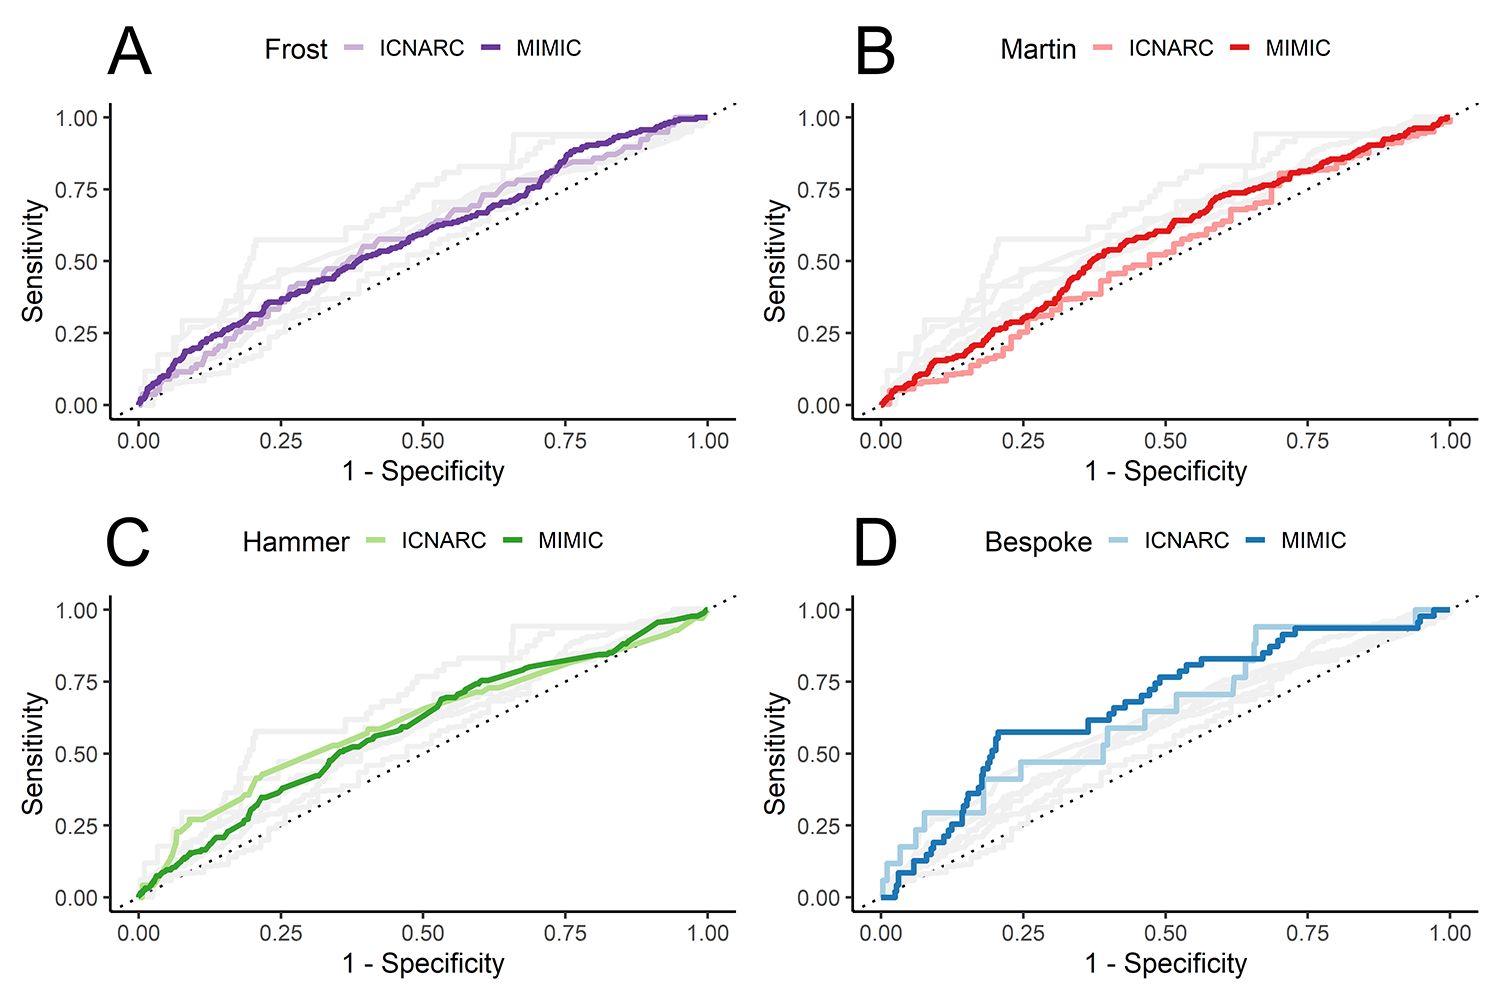
\includegraphics[width=\textwidth]{discrimination.png}
	\caption{Comparison of model discrimination as Reciever Operating Characteristic (ROC) curves. The diagonal dashed line represents an area under the curve of 0.5, that is, a model that essentially guesses between readmission and not at random. The more convex a given curve is away from this diagonal, the greater its discrimination.}
	\label{DiscriminationFig}
\end{figure}

\begin{table*}[h]
\centering
	\renewcommand{\arraystretch}{1.4}
		\caption{Comparisons of model predictive performance. AUC measures discrimination (between 0.5 and 1.0, greater is better), and $\chi^{2}$ measures calibration (lower is better). P-values indicate whether there is a significant difference between observed and expected readmission, thus a value >0.05 indicates good calibration.}
		\begin{tabular}{lllllll}
		\hline
		& MIMIC-III & & & ICNARC & &\\
		Model & AUC & $\chi^{2}$ & \textit{p} & AUC & $\chi^{2}$ & \textit{p}\\
		\hline
		Frost & 0.586 & 138.63 & <0.001 & 0.582 & 4.39 & 0.789\\
		Martin & 0.569 & 75.84 & <0.001 & 0.522 & 26.76 & <0.001\\
		Hammer & 0.589 & 630.23 &  <0.001 & 0.609 & 82.47 & <0.001\\
		Bespoke & 0.675 & 4.72 & 0.787 & 0.643 & 9.91 & 0.271\\
		\hline
		\end{tabular}
	\label{ModelComparisonTable}
\end{table*}


\subsection{Model comparisons}

% Workflow in compare_scores
Readmission risk was predicted for each individual in each dataset using each of the four models in turn. For each model, discrimination was plotted as a ROC curve, and the area under the curve (AUC) was calculated. Calibration was calculated for each model by splitting the dataset into deciles based on the predicted probabilities for a given model. Observed vs expected readmission was then plotted for each decile, and calibration was assessed by the Hosmer-Lemeshow $ \chi^{2} $ test.

\section{Results}

Comparisons of discrimination among models are shown visually in \Cref{DiscriminationFig}, and comparisons of calibration in \Cref{CalibrationFig}. A summary of calibration and discrimination of all models for both datasets can be found in \Cref{ModelComparisonTable}.



For the MIMIC-III dataset, the final model retained sex, age, respiratory rate, and a high-risk surgical speciality (gastrointestinal, vascular or thoracic surgery). For the ICNARC dataset, the final model retained APACHE-II score, severe anaemia, serum lactate levels, out-of-hours discharge, if any amount of respiratory support was required, total days of organ support and whether the patient's lowest Glasgow coma score during their first 24 h.

Discrimination for the published models was poor in both datasets. The two bespoke models showed better discrimination than the published models within each dataset, but still only showed acceptable discrimination (AUC = 0.675 in the MIMIC dataset, AUC = 0.643 in the ICNARC dataset)

\begin{figure}
\centering
	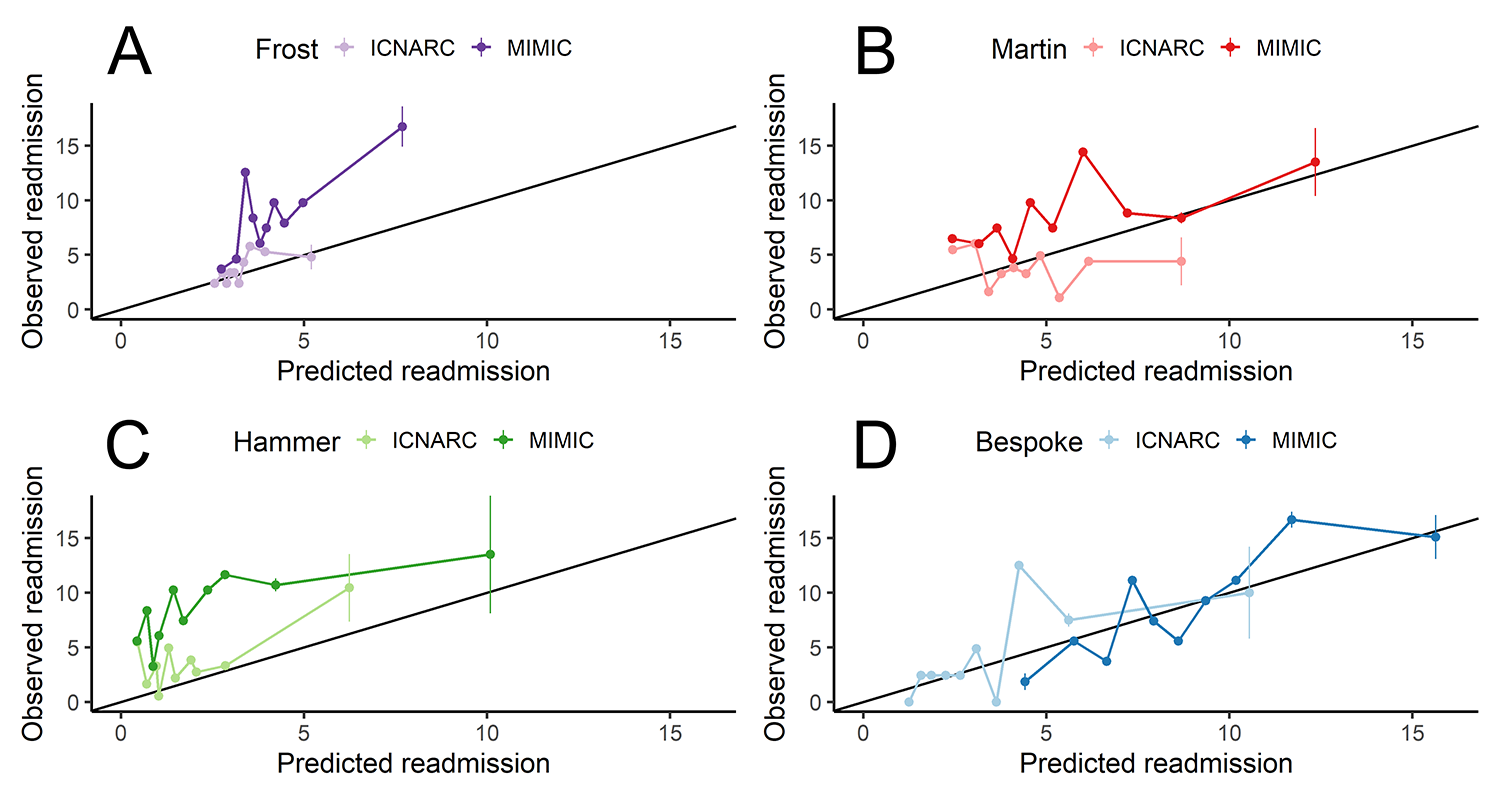
\includegraphics[width=\textwidth]{calibration.png}
	\caption{Comparison of model calibration. For each model, the data is split into deciles based on the model's predicted readmission probabilities, then observed and predicted readmission are compared within each decile. The diagonal black line shows ideal, perfect calibration. Deciles above the line therefore represent the model under-predicting readmission, and deciles below the line represent over-prediction.}
	\label{CalibrationFig}
\end{figure}

Published models also tended to be poorly calibrated in both datasets - only the Frost model was well-calibrated within the ICNARC dataset ($\chi^{2}$ = 4.39, \textit{p} = 0.789), and no published model was well-calibrated to the MIMIC dataset. As would be expected for models fitted using the data at hand, both bespoke models were well-calibrated


\section{Discussion \& Conclusions}

Our findings require consideration within the context of ICU discharge and readmission. Ideally, once a patient is deemed to be clinically stable, they will be discharged from ICU. That decision to discharge is based on physiological and demographic data, which are routinely recorded, but also on clinical impressions which are at best recorded as free text field rather than variables which can feed directly into a model.

Unlike, for example, mortality, discharging a patient from ICU is a \textit{choice} made by skilled clinicians. Not only do clinicians have access to any data that may be contained in datasets like those we used here, but they also may utilise additional data, context, and their clinical intuition. Thus, a clinician's judgement can be thought of as a continuously-updating risk prediction model, and that a patient will not be discharged until clinicians believe their risk of readmission is low. 

As clinicians do not discharge patients from ICU with the expectation that they will be subsequently readmitted, the `readmission' flag within datasets such as these should be more properly interpreted as `residual' readmission. That is, all patients have already been assessed by the `clinician's judgement' risk prediction model, and deemed to be of sufficiently low readmission risk as to be discharged. What readmission risk prediction models are therefore attempting to do is correctly predict those cases that the `clinician's judgement' model incorrectly assigned, using, in most cases, a smaller pool of potential predictor variables with less clinical context than was used in the original assessment. It is unlikely that information of high predictive value for predicting readmission will thus be found in the records of patients who were successfully discharged. This is especially true in the subset of elective surgical admissions that we have studies here, as these tend to be `healthier', relative to the average critical care patient, than unplanned or emergency admissions.

It must be noted that our work is not intended to encourage uptake of either of our bespoke models as risk prediction tools, but instead to highlight that predictive methods using currently available data are unlikely to be able to help clinicians improve decisions on the optimal timing of discharge. Our work can be seen in part as a vote of confidence that ICU staff are indeed highly skilled at predicting readmission risk for individual patients using the data available. This work therefore highlights the difficulty of applying risk prediction models to a process that is already well under the control of clinical staff, and that readmission in this patient population may be inherently unpredictable. 

Instead, it is our hope that this work may discourage future studies from simply fitting ever more complex risk estimation models to routinely-gathered data, and instead focus on collecting additional contextual variables, such as unit occupancy or capacity, that may lend context to the discharge decision and aid capacity planning, or identifying variables which have a causal relationship with readmission, that may provide targets for intervention aimed at lowering risk.


\begin{multicols}{2}
\bibliographystyle{thesis}
{\small
\bibliography{readmission_refs}}

\end{multicols}
\end{document}
